\chapter{Introdução}

\begin{figure}[ht]
	\center
	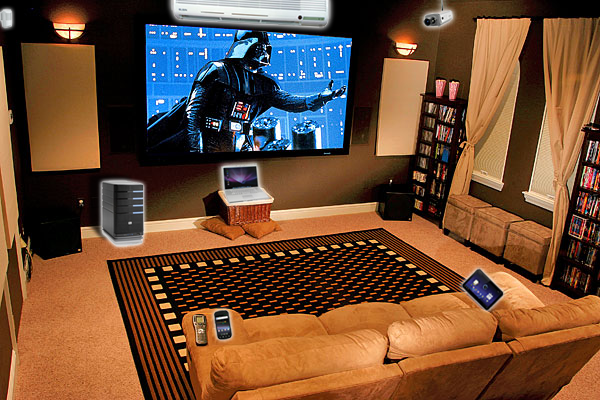
\includegraphics[scale=0.7]{imagens/salaUbiqua}
	\caption{Exemplo de ambiente inteligente.}
	\label{fig:ambienteInteligente}
\end{figure}

A computação ubíqua caracteriza-se por representar ambientes computacionais responsáveis por realizar determinadas tarefas predeterminadas de tal forma que certas premissas sejam obedecidas. Tais ambientes são normalmente compostos por um \emph{middleware} e diversas outras aplicações externas. Ao primeiro, cabe tratar e abstrair os detalhes das camadas inferiores e orquestrar as interações entre os diversos dispositivos espalhados pelo ambiente, enquanto que as aplicações devem tratar as interações realizadas junto aos usuários. É necessário que os componentes desse tipo de sistema trabalhem harmonicamente a fim de evitar, sempre que possível, toda e qualquer intervenção humana. A esta característica dá-se o nome de invisibilidade ~\cite{gomes2007, weiser1993, weiser1999}. Faz-se necessário, inclusive, que tais sistemas sejam pró-ativos ~\cite{gomes2007, buzeto2010} e consigam determinar, com a ajuda de informações de contexto previamente coletadas, quais as melhores decisões a serem tomadas em determinados instantes. Deve-se considerar, ainda, a mobilidade ~\cite{gomes2007, buzeto2010, weiser1999} dos aparelhos presentes e regidos dentro do ambiente em questão, a saber, o \emph{smart space}.

\begin{comment}
Em um ambiente inteligente se faz necessária a adaptabilidade de serviços de forma transparente para os clientes, ou seja, caso um serviço não esteja mais sendo provido por determinado dispositivo, o \emph{smart space} deve identificar esta falha e procurar um outro servidor ~\cite{gomes2007, passarinho2008, paranhos2009}.
\end{comment}

\begin{comment}
\section{DSOA}

Com o objetivo de auxiliar a modelagem de um \emph{smart space} levando em consideração as características de um ambiente ubíquo, foi criada a arquitetura DSOA(\emph{Device Service Oriented Architecture})~\cite{buzetoDSOA2010} que faz uso dos conceitos definidos na SOA(\emph{Service Oriented Architecture}) aplicados a um ambiente inteligente, onde recursos e serviços estarão disponíveis de forma dinâmica. Recursos, segundo a definição na proposta da DSOA, são um grupo de funcionalidades logicamente relacionadas que deverão ser acessíveis por meio de interfaces pré-definidas ~\cite{buzeto2010}. 

Esses recursos serão acessados por meio do \emph{middleware} \emph{uOS}, que utiliza um conjunto de protocolos \emph{uP} (\emph{Ubiquitous Protocols}) como interface de comunicação com \emph{drivers} de recursos disponíveis. A infra-estrutura implementada pelo \emph{uOS} para gerir os recursos do ambiente permite que uma aplicação de um dispositivo acesse recursos, apresentados na forma de um \emph{driver} (\emph{UosDriver}) de outros dispositivos presentes no ambiente.

Quando uma aplicação solicita um serviço de algum recurso, o \emph{uOS} deve tomar uma decisão sobre qual será o dispositivo detentor de tal recurso que provê o serviço solicitado que irá ser escolhido. Para que o \emph{uOS} possa tomar uma decisão inteligente sobre a escolha do dispositivo detentor do recurso, deseja-se que o tipo do recurso seja conhecido. Atualmente, a arquitetura DSOA/\emph{uOS} é pouco maleável nessa definição de tipo de recursos. Os recursos são definidos de forma linear, por exemplo: um recurso de \emph{mouse} com dois botões possui um \emph{driver} associado, já um \emph{mouse} com três botões, possui um outro \emph{driver} associado que não possui nenhuma relação com o primeiro, o que dificulta a tomada de decisão por parte do \emph{middleware}. Existem diversos padrões definidos que fazem uso de uma classificação de dispositivos ou recursos, mas não se adequam à arquitetura DSOA.

O objetivo deste trabalho é definir uma classificação de recursos e a partir desta classificação, prover uma hierarquia de recursos extensível para a arquitetura DSOA do \emph{middleware} de Computação Ubíqua \emph{uOS}. Essa hierarquia irá facilitar a escolha de determinado serviço provido por algum recurso por parte do \emph{uOS} ou de alguma aplicação cliente.
\end{comment}

Este trabalho está organizado da seguinte maneira: O capítulo 2 fundamenta os conceitos que serão utilizados neste trabalho. É iniciado apresentando uma visão geral do projeto UbiquitOS, explicando os principais conceitos da DSOA e mostrando em detalhes os protocolos que constituem o \emph{uP}. A seção seguinte mostra a importância da classificação de recursos bem como as diferentes maneiras de se classificar e representá-la. Ainda na segunda seção, serão apresentados alguns dos principais padrões conhecidos e projetos de Computação Ubíqua que utilizam uma classificação de recursos ou dispositivos para auxiliar em suas atividades. A seção e o capítulo são finalizados realizando um comparativo entre as diferentes classificações apresentadas. No capítulo 3 será apresentada a proposta de classificação deste trabalho e os impactos na arquitetura DSOA/\emph{uOS} e em seus protocolos.